\documentclass[11pt,a4paper,twoside,openright]{report}

%frontespizio
\providecommand{\coursename}{Progetto di Ingegneria Informatica}
\providecommand{\annoacc}{2013-2014}
\providecommand{\principaladviser}{Prof. Andrea Bonarini}
\providecommand{\firstauthor}{Davide Tateo}
\providecommand{\firstauthorid}{799311}
\title{Cognitive SLAM: knowledge-based self-localization and mapping}
\author{\firstauthor}

\usepackage{settings/frontesp}

\usepackage{hyperref}
\hypersetup{
    colorlinks,
    citecolor=black,
    filecolor=black,
    linkcolor=black,
    urlcolor=black
}

\usepackage{tabularx}
\usepackage{subfigure}
\usepackage{afterpage}
\usepackage{amsmath,amssymb}            
\usepackage{rotating}  
\usepackage{fancyhdr}  
\usepackage[scriptsize]{caption} 
\hyphenation{a-gen-tiz-za-zio-ne}

%\setlength{\paperwidth}{16cm}
%\setlength{\paperheight}{24cm}
\setlength{\oddsidemargin} {2. cm}
\setlength{\evensidemargin} {2. cm}
\addtolength{\oddsidemargin} {-0.4 cm}
\addtolength{\evensidemargin} {-0.4 cm}
\linespread{1.1}

\usepackage[italian]{babel}
\usepackage[latin1]{inputenc}
\renewcommand{\captionfont}{\normalfont \sffamily \itshape \small}

\pagestyle{empty}

\begin{document}
\titlep
\thispagestyle{empty} \normalfont \cleardoublepage
\vspace{17cm}

%\large
\begin{flushright}
\itshape{A mio papà\dots}
\end{flushright}

\thispagestyle{empty}  \cleardoublepage
\pagenumbering{Roman}
\newpage
\chapter*{Sommario}

\addcontentsline{toc}{chapter}{Sommario}

Lo SLAM � uno dei principali problemi nello sviluppo di robot autonomi. Gli approcci correnti sono afflitti da un pesante costo computazionale e si comportano male in abienti dinamici e disordinati; le performance di questi sistemi diventano ancora peggiori se si utilizzano sensori a basso costo, necessari per le applicazioni commerciali.
Questa tesi affronta il problema da un punto di vista nuovo e originale, usando feature ad alto livello come punti chiave e sfruttando la conoscenza di un esperto e un linguaggio fuzzy per riconoscerli, per tenere traccia di punti chiave forti e stabili e permettere mappe pi� intelligenti e una localizzazione robusta in ambienti complessi. L'idea fondamentale � quella di mantenere il tasso di errore della localizzazione limitato e ridurre il costo necessario a far navigare con successo un robot autonomo in un ambiente interno, usando solo i dati provenienti da una webcam e una unit� di misura inerziale a basso costo.
Il principale problema � il riconoscimento di feature ad alto livello, come porte e scaffali, affrontato tramite un classificatore fuzzy ad albero, definito da un esperto, in modo da evitare fasi di allenamento e migliorare la generalit� del riconoscimento.

\chapter*{Abstract}

\addcontentsline{toc}{chapter}{Abstract}

SLAM is one of the key issues in autonomous robots development. Current approaches are affected by heavy computational load and misbehave in cluttered and dynamic environment; their performance get even worse with low cost sensors, needed for market applications.
This thesis faces the problem in a new and original way, working with high level features as key points and using expert knowledge and a fuzzy language to detect them, in order to track strong and stable key points and allow smarter maps and robust localization in complex environments. The key idea is to keep the error rate of the localization process limited, and to reduce the cost of an autonomous robot to successfully navigate into an indoor environment using only the data from a webcam and a low cost Inertial measurement unit.
The main issue is the high level feature recognition, like doors and shelves, done by an expert-defined fuzzy tree classifier, in order to avoid training and improve generalization of recognition.
\thispagestyle{empty} \vspace*{.75truecm} \cleardoublepage
\tableofcontents
\clearpage
\chapter*{Ringraziamenti}

\addcontentsline{toc}{chapter}{Ringraziamenti}

Ringrazio ................

\thispagestyle{empty} \vspace*{.75truecm} \normalfont \cleardoublepage
\pagestyle{plain}\renewcommand{\chaptermark}[1]{\markboth{\chaptername\ \thechapter.\ #1}{}} 
\renewcommand{\sectionmark}[1]{\markright{\thesection.\ #1}}         
\fancyhead[LE,RO]{\bfseries\thepage}    
                                        
\fancyhead[RE]{\bfseries\leftmark}    
\fancyhead[LO]{\bfseries\rightmark}     
\renewcommand{\headrulewidth}{0.3pt} 
\pagenumbering{arabic}
\thispagestyle{plain}

\chapter{Introduzione}
\label{Introduzione}
\thispagestyle{empty}

\begin{quotation}
{\footnotesize
\noindent{\emph{``Qualunque cosa che accade, accade'' \\
``Qualunque cosa che, accadendo, ne fa accadere un'altra, ne fa accadere un'altra.'' \\
``Qualunque cosa che, accadendo, induce se stessa a riaccadere, riaccade.'' \\
``Per� non � detto che lo faccia in ordine cronologico.''
}
}
\begin{flushright}
Douglas Adams, Mostly Harmless
\end{flushright}
}
\end{quotation}
\vspace{0.5cm}

\section{Inquadramento generale}
Uno dei problemi chiave della robotica � la localizzazione di un robot in un ambiente sconosciuto. Questo problema � noto come ``SLAM'', Simultaneus localization and Mapping, ed � attualmente una delle aree pi� importanti della ricerca riguardante i robot autonomi. 
In particolare, questo problema risulta ancora pi� difficile se applicato a robot dotati di sensori a basso costo, quali webcam e unit� di misura inerziale economiche, restrizione fondamentale per la diffusione di applicazioni di robotica autonoma nel mondo reale.
Lo scopo della tesi � di sviluppare un framework per risolvere il problema della localizzazione di robot autonomi dotati di sensori a basso costo, quali ad esempio i quadricotteri



La prima parte contiene una frase che spiega l'area generale dove si svolge il lavoro; una che spiega la sottoarea pi\`u specifica dove si svolge il lavoro e la terza, che dovrebbe cominciare con le seguenti parole ``lo scopo della tesi \`e \dots'', illustra l'obbiettivo del lavoro. Poi vi devono essere una o due frasi che contengano una breve spiegazione di cosa e come \`e stato fatto, delle attivit\`a� sperimentali, dei risultati ottenuti con una valutazione e degli sviluppi futuri. La prima parte deve essere circa una facciata e mezza o due

\section{Breve descrizione del lavoro}
La seconda parte deve essere una esplosione della prima e deve quindi mostrare in maniera pi\`u esplicita l'area dove si svolge il lavoro, le fonti bibliografiche pi\`u importanti su cui si fonda il lavoro in maniera sintetica (una pagina) evidenziando i lavori in letteratura che presentano attinenza con il lavoro affrontato in modo da mostrare da dove e perch\'e \`e sorta la tematica di studio. Poi si mostrano esplicitamente le realizzazioni, le direttive future di ricerca, quali sono i problemi aperti e quali quelli affrontati e si ripete lo scopo della tesi. Questa parte deve essere piena (ma non grondante come la sezione due) di citazioni bibliografiche e deve essere lunga circa 4 facciate.

\section{Struttura della tesi}
La terza parte contiene la descrizione della struttura della tesi ed \`e organizzata nel modo seguente.
``La tesi \`e strutturata nel modo seguente.

Nella sezione due si mostra \dots

Nella sez. tre si illustra \dots

Nella sez. quattro si descrive \dots

Nelle conclusioni si riassumono gli scopi, le valutazioni di questi e le prospettive future \dots

Nell'appendice A si riporta \dots (Dopo ogni sezione o appendice ci vuole un punto).''

I titoli delle sezioni da 2 a M-1 sono indicativi, ma bisogna cercare di mantenere un significato equipollente nel caso si vogliano cambiare. Queste sezioni possono contenere eventuali sottosezioni.

%``Terence: "Mi fai un gelato anche a me? Lo vorrei di pistacchio" \\
%Bud: "Non ce l'ho il pistacchio. C'ho la vaniglia, cioccolato, fragola, limone e caff�"\\
%Terence: "Ah bene. Allora fammi un cono di vaniglia e di pistacchio"\\
%Bud: "No, non ce l'ho il pistacchio. C'ho la vaniglia, cioccolato, fragola, limone e caff�"\\
%Terence: "Ah, va bene. Allora vediamo un po', fammelo al cioccolato, tutto coperto di pistacchio"\\
%Bud: "Ehi, macch� sei sordo? Ti ho detto che il pistacchio non ce l'ho!"\\
%Terence: "Ok ok, non c'� bisogno che t'arrabbi, no? Insomma, di che ce l'hai?"\\
%Bud: "Ce l'ho di vaniglia, cioccolato, fragola, limone e caff�!"\\
%Terence: "Ah, ho capito. Allora fammene uno misto: mettici la fragola, il cioccolato, la vaniglia, il limone e il caff�. Charlie, mi raccomando il pistacchio, eh"''}

\chapter{Stato dell'arte}
\label{capitolo2}
\thispagestyle{empty}

\begin{quotation}
{\footnotesize
\noindent{\emph{Doc: Ecco perché non ha funzionato: c'è scritto ``Made in Japan''. \\
Marty: E che vuol dire Doc? Tutta la roba migliore è fatta in Giappone. \\
Doc: Incredibile!
} }
\begin{flushright}
Ritorno al Futuro, parte III
\end{flushright}
}
\end{quotation}
\vspace{0.5cm}

\section{SLAM}

Il problema della localizzazione di un robot in un ambiente sconosciuto è stato affrontato fin dagli anni 90' a partire da \cite{174711}, articolo nel quale per la prima volta si delineava un framework per localizzare un robot costruendo contemporaneamente la mappa dell'ambiente.
Tramite l'utilizzo di sonar, venivano estratte feature geometriche con cui veniva costruita la mappa, nella quale il robot si localizzava. 
Il problema principale della localizzazione è il ``problema della correlazione'': se la posizione della feature rispetto alla quale ci si localizza è affetta da incertezza, la conseguente stima della posizione effettuata rispetto a tale feature sarà affetta da un errore che dipende dall'errore della posizione della feature stessa. 
Questo problema diventa tanto più grave se si pensa che la posizione del robot in ogni istante non è nota a priori, ma deve essere stimata sulla base delle osservazioni precedenti. 
Come è facile vedere, è necessario risolvere questo problema per evitare che l'errore della generazione della mappa e l'errore della stima della posizione divergano nel tempo. 
Per risolverlo, gli autori hanno utilizzato un filtro di Kalman esteso.

Come è noto, il filtro di Kalman è uno stimatore Bayesiano ricorsivo, che, supposto noto il modello lineare che regola la generazione dei dati e la loro osservazione, supposto che l'errore di misura e di modello siano gaussiani, restituisce la densità di probabilità del sistema osservato. 
Il filtro di Kalman, se utilizzato secondo le ipotesi, è uno stimatore ottimo dello stato del sistema osservato, secondo i minimi quadrati.
Tuttavia, nell'ambito della robotica, e in particolare nel problema della localizzazione, il modello di generazione e osservazione dei dati non può essere considerato lineare.
E' quindi necessario utilizzare un'estensione del filtro di Kalman al caso non lineare: il filtro di Kalman esteso (EKF) è una delle possibili soluzioni al problema. 
L'idea alla base del filtro di Kalman esteso è quella di lavorare sul modello linearizzato, stimato ricorsivamente dal modello non lineare sulla base della stima corrente.

Per avere una buona stima della posizione è necessario utilizzare un gran numero di feature, numero che cresce molto rapidamente con l'aumentare della dimensione dell'ambiente.
La complessità computazionale dell'approccio tradizionale basato sul filtro di Kalman esteso è $\mathcal{O}(N^3)$, con $N$ numero di feature, e quindi il tempo di calcolo diventa ben presto inaccettabile.
Per risolvere questo problema è stato introdotto in \cite{Montemerlo02a}  un nuovo algoritmo detto FastSLAM, che consiste nell'utilizzo del Particle Filter, e del filtro di Kalman esteso in combinazione. L'algoritmo associa ad ogni feature considerata, un filtro di Kalman esteso; la densità di probabilità congiunta, invece, viene calcolata sfruttando il Particle filter. 
Il Particle Filter è un altro stimatore Bayesiano ricorsivo, che, invece di un modello e dell'assunzione di rumore gaussiano, sfrutta metodi di tipo Monte Carlo per stimare la densità di probabilità del sistema che genera i dati.
Il risultato è un algoritmo che ha complessità computazionale $\mathcal{O}(N\log M)$, con $M$ numero di feature e $N$ è il numero di particelle usate dal Particle Filter. 
Questo approccio rende il problema trattabile nella maggior parte dei casi, pur essendo pesante computazionalmente, essendo necessario un elevato numero di particelle per avere una buona localizzazione.

Vista la particolarità del problema quando il sensore utilizzato è una videocamera monoculare, sono stati sviluppati algoritmi ad hoc.
Uno degli algoritmi più usati è PTAM, descritto in \cite{klein07parallel} e \cite{klein08improving}.
L'idea alla base di questo algoritmo è dividere in due thread separati il tracking e la creazione della mappa: un thread si occupa del tracking robusto di feature a basso livello, mentre l'altro thread si occupa della creazione della mappa. 
Per rendere efficiente il processo di mapping, solo i keyframe, ossia i frame che contengono maggiore informazione rispetto a quella già presente, vengono considerati.
Per rendere il processo di mapping robusto, vengono utilizzate tecniche batch per costruire la mappa, come ad esempio il bundle adjustment.
PTAM, tuttavia, nasce per applicazioni di realtà aumentata, e quindi necessita di una inizializzazione, per risolvere i problemi dell'acquisizione del primo keyframe e per gestire la scala della mappa.

Un altro approccio alternativo è quello di usare tutti i dati dell'immagine per eseguire la localizzazione, questo approccio è alla base ad esempio di DTAM, Dense Tracking and Mapping, descritto in \cite{conf/iccv/NewcombeLD11}.

Si sono dimostrati efficaci anche i metodi semi-diretti, come SVO, Semi Direct Visual Odometry, un algoritmo che riesce a ottenere altissime prestazioni limitando l'estrazione delle feature ad alto livello ai soli keyframe, operando direttamente sulle intensità dei pixel nei frame successivi, eliminando le fasi computazionalmente più onerose, che sono l'estrazione e l'abbinamento delle feature. SVO si basa sulle idee di PTAM, ma migliora sia le prestazioni, riuscendo a essere computazionalmente più leggero, sia la precisione della mappa e della localizzazione riducendo di molto gli outlier.

\section{Riconoscimento di Oggetti}

La quasi totalità degli algoritmi di riconoscimento di oggetti nell'immagine è basata su tecniche di machine learning.
Una delle classi di algoritmi più usati sono quelli basati sulle Haar-like feature, descritte in \cite{710772}.
Queste feature sono calcolate in aree rettangolari, all'interno delle quali vengono sommati i valori dell'intensità dei pixel. Le somme sono in seguito usate per calcolare differenze tra aree di interesse, per poter riconoscere feature geometriche quali angoli, linee o bordi.
Un efficiente algoritmo per il riconoscimento di oggetti è descritto in \cite{Viola01rapidobject} ed è stato ampliato in \cite{Lienhart02anextended}, e consiste nell'utilizzare in cascata una serie di classificatori via via più restrittivi; ognuno dei classificatori di ogni stadio è costruito attraverso una tecnica di boosting, ossia sono formati da un insieme di classificatori deboli che creano un classificatore complessivo più restrittivo. I classificatori di base sono solitamente alberi di decisione. Il classificatore complessivo da una risposta binaria, per riconoscere effettivamente l'oggetto deve essere applicato tramite una finestra mobile su tutta l'immagine. \\
Un algoritmo simile può essere trovato in \cite{journals/ijista/AbramsonSG07}, dove però invece che feature Haar-like, vengono utilizzati direttamente un insieme di pixel nell'immagine.

Un'altra importante classe di algoritmi è basato sulle feature HOG (Histogram of Oriented Gradients). Queste feature sono ricavate contando le occorrenze dell'orientamento dei gradienti in sotto blocchi dell'immagine.
Su queste feature si basa l'algoritmo descritto in \cite{lsvm-pami}. Questo algoritmo è in grado di definire un oggetto a partire dalle sue parti, e quindi è robusto anche a occlusioni parziali dell'oggetto. Tuttavia è computazionalmente molto più pesante dell'approccio basato su feature Haar-like.

Più recenti sono i metodi basati sul deep learning. Tra questi, i più promettenti nel riconoscimento di oggetti sono basati sulle reti neurali convoluzionali. La particolarità di queste reti è di essere basata su kernel di nodi collegati in maniera fissa, e ripetuti per coprire tutta l'immagine. La struttura rigida sfrutta la località dell'informazione nell'immagine, e permette un training più efficiente.
Un esempio di applicazione si può trovare in \cite{NIPS2012_4824}.

%%TODO bag of words?

\section{Reasoning}

I sistemi esperti sono stati per lungo tempo una delle branche dell'intelligenza artificiale più attive. 
In particolare si può citare il noto strumento per la creazione di sistemi esperti, CLIPS, e la sua estensione alla logica fuzzy, FuzzyCLIPS. Entrambi permettono di descrivere delle classi di oggetti e di definire predicati tra di essi, in modo da poter compiere inferenza sui dati in ingresso.
La ricerca sui sistemi di deduzione formale tuttavia si è spostata da i sistemi esperti al web semantico.
L'attuale standard per i sistemi di inferenza è il linguaggio OWL 2, descritto in \cite{owl2-overview} e \cite{owl2-primer}, linguaggio fortemente basato sulle logiche descrittive che permettono un buon compromesso tra espressività, complessità computazionale e mantengono la logica utilizzata decidibile.
Un esempio di reasoning applicato al riconoscimento delle immagini può essere trovato in \cite{DBLP:journals/ivc/MaillotT08}, in cui feature a basso livello vengono estratte da un meccanismo di machine learning, e utilizzate da un sistema di inferenza che sfrutta una ontologia per l'analisi ad alto livello dell'immagine.

\chapter{Concetti Fondamentali}
\label{cap:concetti}
\thispagestyle{empty}

\begin{quotation}
{\footnotesize
\noindent{\emph{Doc: Ovviamente il continuum temporale è stato interrotto creando questa nuova temporale sequenza di eventi risultanti in questa realtà alternativa. \\
Marty: Che lingua è Doc? \\
Doc: Ah si, si, si, si, si! Lascia che ti spieghi. Immagina, che questa linea rappresenti il tempo\dots}}
\begin{flushright}
Ritorno al Futuro, parte II
\end{flushright}
}
\end{quotation}
\vspace{0.5cm}

Si illustrano di seguito i concetti fondamentali alla comprensione della tesi.

\section{Logica Fuzzy}
La logica fuzzy è una logica multivalore che permette di esprimere non solo la verità o la falsità di una affermazione, ma anche il suo valore di verità, che può essere qualsiasi numero tra 0 (ossia l'afefrmazione è falsa) e 1 (ossia l'affermazione è vera).

Grazie a questa logica è possibile esprimere concetti che in una logica a due valori sono paradossali.
Ad esempio, la frase ``sono un bugiardo'', che nella logica a due valori risulta paradossale, nella logica fuzzy essa può assumere valori consistenti.

\subsection{Insiemi Fuzzy}
La logica fuzzy è basata fortemente sul concetto di insieme fuzzy. Un insieme fuzzy è un insieme la cui funzione di appartenenza può avere valori nell'intervallo $[0, 1]$.
I fuzzy set sono quindi definiti da una funzione di appartenenza $f$ definita su un dominio $D$, avente come codominio l'intervallo $[0,  1]$.  Formalmente un fuzzy et è definito come:

\begin{equation*}
 f:D\leftarrow [0, 1]
\end{equation*}

Si definisce altezza di un insieme fuzzy il massimo grado di verità possibile per un elemento.
Un fuzzy set si dice normale se la sua altezza è pari a uno.

Un fuzzy set si dice unimodale se esiste un unico insieme in cui le variabili hanno valore di verità pari a 1.


%%TODO qui?? forse da spostare...
Si definisce variabile linguistica $X$, definita sulla variabile di base $u$ una tupla così definita:
\begin{equation*}
$(X, T(X), U, G, M)$
\end{equation*}

dove:

\begin{description}
 \item [X] è il nome della variabile.
 \item [T(X)] è un insieme di termini, detti anche valori linguistici.
 \item [U] è il dominio della variabile di base $u$.
 \item [G] è una regola sintattica per generare l'interpretazione X per ogni valore di u.
 \item [M] è una regola semantica che associa a X il suo significato.
\end{description}


Data una variabile $x$, è possibile definire più fuzzy set rispetto al suo dominio. Si parla di frame of cognition quando valgono le seguenti condizioni:
\begin{enumerate}
 \item L'intero dominio della variabile è coperto da almeno un fuzzy set con valore di verità maggiore di zero.
 \item Tutti i fuzzy set sono unimodali.
 \item Tutti i fuzzy set sono normali.
\end{enumerate}

Inoltre si parla di partizione fuzzy, se la somma delle funzioni di appartenenza di ogni fuzzy set in ogni punto del dominio è uguale a 1.

La normale teoria degli insiemi è contenuta nella teoria degli insiemi fuzzy: Infatti un intervallo è un insieme fuzzy, con valore di verità di tutti gli elementi pari a 1. Anche i singoli elementi possono essere trattati, tramite il fuzzy set singleton, che ha valore di verità 1 per un solo elemento del dominio, e 0 per tutti gli altri.

\subsection{Operazioni sui fuzzy set}

Sui fuzzy set sono definite le seguenti operazioni:
\begin{itemize}
 \item unione
 \item intersezione
 \item complemento
\end{itemize}

\subsubsection{Complemento}

Dato un insieme fuzzy $A$, con funzione di appartenenza $\mu_A$ il complemento è definito come:

\begin{equation*}
 c(\mu_A(x)) = \mu_{\neg A}(x)
\end{equation*}

Il complemento di insiemi fuzzy deve rispettare i seguenti assiomi:
\begin{enumerate}
 \item $c(0)=1$, $c(1)=0$ (condizioni al contorno)
 \item $c$ è una funzione continua.
 \item $c$ è involutiva, ossia $c(c(a))=a\, \, \forall a \in [0, 1]$
\end{enumerate}

l'unica funzione che rispetta i seguenti assiomi è la funzione:

\begin{equation*}
 c(x) = 1 - x
\end{equation*}

\subsubsection{Intersezione}

Dati due insiemi fuzzy $A$ e $B$, con funzione di appartenenza $\mu_A$ e $\mu_B$ l'intersezione  è definita come:

\begin{equation*}
 i(\mu_A(x), \mu_B(x)) = \mu_{A\cap B}(x)
\end{equation*}

L'intersezione di insiemi fuzzy deve rispettare i seguenti assiomi:

\begin{enumerate}
 \item $i(a, 1)=a$ (condizioni al contorno)
 \item $d\geq b \implies  i(a,d)\geq i(a,b)$ (monotonicità)
 \item $i(b,a) = i(a,b)$ (commutatività)
 \item $i(i(a,b),d)=i(a,i(b,d))$ (associatività)
 \item $i$ è una funzione continua
 \item $a\geq i(a,a)$ (sub-idempotenza)
 \item $a_1<a_2 \wedge b_1<b_2\implies i(a_1,b_1)<i(a_2,b_2)$ (monotonicità stretta)
\end{enumerate}

Non esiste un'unica funzione che rispetta questi assiomi. Ogni funzione che rispetta questi assiomi viene detta T-norm.
Esempi di T-norm sono l'operatore minimo e il prdotto tra i valori di verità.

\subsubsection{Unione}

Dati due insiemi fuzzy $A$ e $B$, con funzione di appartenenza $\mu_A$ e $\mu_B$ l'unione è definita come:

\begin{equation*}
 u(\mu_A(x), \mu_B(x)) = \mu_{A\cup B}(x)
\end{equation*}

L'unione di insiemi fuzzy deve rispettare i seguenti assiomi:

\begin{enumerate}
 \item $u(a, 0)=a$ (condizioni al contorno)
 \item $b \leq d implies u(a,b) \leq u(a,d)$ (monotonicità)
 \item $u(a,b) = u(b,a)$ (commutatività)
 \item $u(a,u(b,d)) = u(u(a,b),d)$ (associatività)
 \item $u$ è una funzione continua
 \item $u(a,a) \geq a$ (super-idempotenza)
 \item $a_1< a_2 \wedge b_1 < b_2 \implies u(a_1,b_1)<u(a_2,b_2)$ (monotonicità stretta)
\end{enumerate}

Non esiste un unica funzione che rispetta questi assiomi. Ogni funzione che rispetta questi assiomi viene detta T-conorm, o S-norm.
Esempi di S-norm sono l'operatore massimo e la somma probabilistica tra i valori di verità.
La somma probabilistica $p$ tra due variabili $a$  e $b$ è definita come:

\begin{equation*}
 p = a+b - a\cdot b 
\end{equation*}

%%TODO aggregazione???

% μA(x) = h[μA1(x), ..., μ An(x)]
% Axioms:
% 1. h[0,..., 0]=0, h[1,..., 1]=1 (boundary conditions)
% 2. monotonicity
% 3. h is continuous
% 4. h(a,..,a) = a (idempotency)
% 5. simmetricity
% Example of aggregation operator: generalized average
% h(a1, ..., an) = (a1α + ...+ anα) 1/α / n


\subsection{Regole Fuzzy}

Una regola di inferenza fuzzy può essere considerata come un modello, un mezzo per definire una funzione tra un ingresso e una uscita.

Le regole fuzzy che consideriamo sono composte nel seguente modo:
\begin{verbatim}
 IF <antecedente> THEN <consequente>
\end{verbatim}

Dove l'antecedente è una formula logica ben formata è il conseguente è una o più proposizioni legate dall'operatore and.

Una formula ben formata è definita come:

\begin{itemize}
 \item Una proposizione è una formula ben formata
 \item Se ``A'' è una formula ben formata, anche ``not A'' è una formula ben formata.
 \item Se ``A'' e ``B'' sono formule ben formate anche ``A and B'', ``A or B'' sono formule ben formate.
 \item null'altro è una formula ben formata.
\end{itemize}

Una proposizione è definita come 

\chapter{Architettura del Sistema}
\label{capitolo4}
\thispagestyle{empty}

\begin{quotation}
{\footnotesize
\noindent \emph{}
\begin{flushright}
\end{flushright}
}
\end{quotation}
\vspace{0.5cm}

In questo capitolo descriveremo l'architettura del sistema implementato. Il sistema è stato progettato in maniera modulare per una serie di motivi: questo tipo di architettura permette di riutilizzare i moduli sviluppati, di estendere semplicemente il sistema con altri moduli, di sostituire eventualmente un intero modulo con un altro che compia le stesse funzioni, di comunicare in maniera semplice con altri sistemi. 

Per raggiungere qusto scopo, si è deciso quindi di utilizzare il middleware ROS (Robot Operating System)~\cite{quigley2009ros}.
ROS è un middleware che, oltre ad offrire molti tool utili per lo sviluppo di complesse applicazioni robotiche, implementa due pattern architetturali importanti, entrambi usati nel nostro lavoro: il pattern publish-subscribe e il pattern client-server.
Questi due patten sono implementati rispettivamente tramite messaggi e servizi: i messaggi definiscono un formato comune per la pubblicazione di dati in topic, i servizi invece specificano un'interfaccia per le chiamate a procedure remote, dichiarando gli input e gli output tra client e server.
Ogni processo che viene eseguito in ROS è chiamato nodo. Per eseguire qualsiasi sistema basato su ros, devono essere presenti tre ulteriori nodi: il nodo Master, che si occupa di garantire la comunicazione tra gli altri nodi, tramite i due pattern supportati, il server dei parametri, che implementa un dizionario condiviso accessibile tramite la rete, in cui i nodi posssono memorizzare e recuperare parametri usati dai loro algoritmi a runtime, il nodo rosout, che si occupa di mantenere i log prodotti dalle appliazioni.

Il sistema sviluppato è pensato per interagire con qualsiasi tipo di robot che sia provvisto di una videocamera monoculare e una unità di misura inerziale (IMU) tramite le due interfacce standard di ROS.
Esse consistono in tre topic: ``imu'', per i dati provenienti dall unità di misura inerziale, ``image\_raw'', per l'immagine proveniente dalla videocamera, ``camera\_info'', che contiene i parametri intrinseci della videocamera, tra cui la matrice di calibrazione della videocamera utilizzata, necessaria per il funzionamento del sistema.
I dati estratti dall'unità di misura inerziale devono essere riferiti al sistema di coordinate della videocamera, infatti l'algoritmo di visione implementato utilizza i dati provenienti dalla IMU per stimare approssimativamente la posa della telecamera.
%TODO sarebbe bello non avere questo vincolo, purchè sia nota la trasformazione dal sistema di coordinate della imu al sistema di coordinate della telecamera. Provo a implementarlo, dovrebbe essere semplice... c'è già il tpic di tf con le opportune trasformazioni...

\section{Diagramma del sistema}

L'architettura del sistema implementato è descritta in \autoref{fig:architettura-sistema}. \\
\begin{figure}[here]
  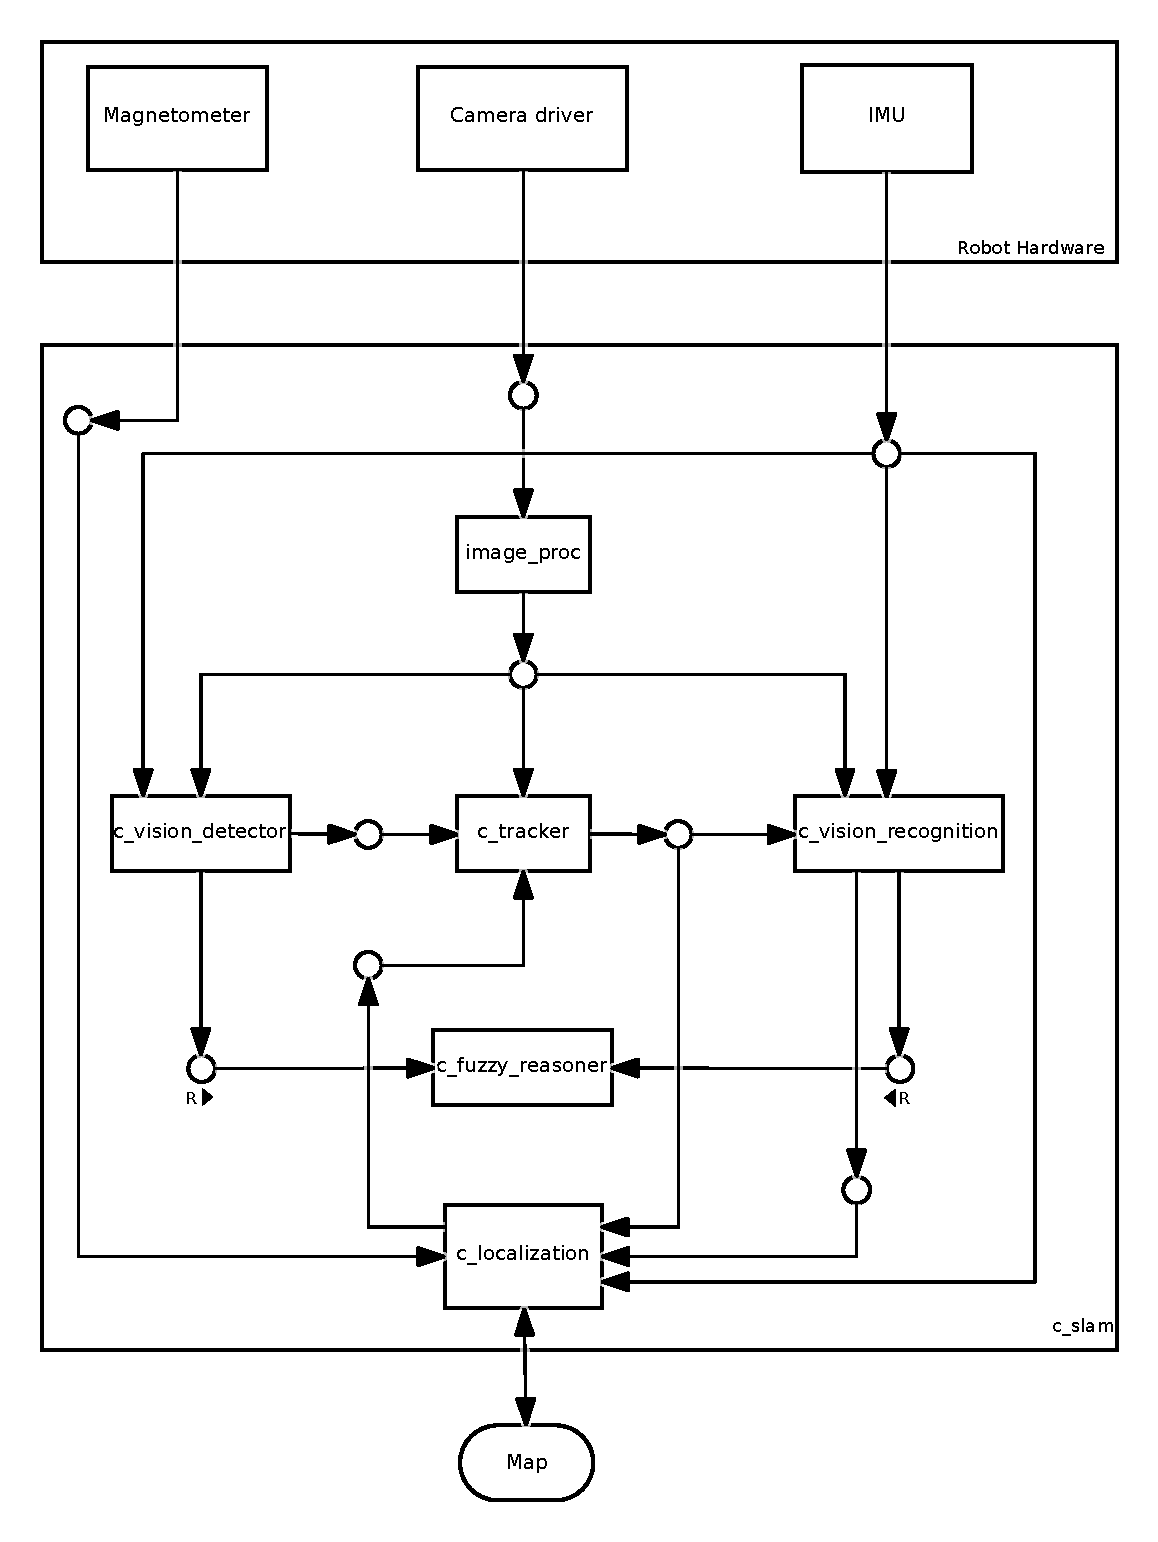
\includegraphics[width=0.9\textwidth]{diagrammi/Sistema}
  \caption{Architettura del sistema implementato}
  \label{fig:architettura-sistema}
\end{figure}


Il diagramma rappresenta i nodi del sistema, segue una breve descrizione di ogni elemento per specificare la loro funzione:

\begin{description}
  \item [image\_proc] si occupa di eliminare la distorsione radiale della videocamera causata dalla curvatura della lente.
  \item [c\_vision\_detector] si occupa di estrarre possibili feature dall'immagine.
  \item [c\_tracking] si occupa di seguire le feture a basso livello estratte dal nodo ``c\_vision\_detector'' nell'immagine, mantenendo un modello in modo da riuscire a riconoscere la feature anche dopo essere stata persa. 
  \item [c\_vision\_slam] si occupa dell'analisi approfondita delle feature, in modo da determinare il tipo di oggetto e la sua posizione nello spazio. 
  \item [c\_fuzzy\_reasoner] implementa un reasoner fuzzy; data una base di conoscenza e un classificatore, analizza le feature in ingresso e le classifica. 
\end{description}




\chapter{Architettura del sistema}
\label{capitolo5}
\thispagestyle{empty}

\begin{quotation}
{\footnotesize
\noindent \emph{``Terence: Ma scusa di che ti preoccupi, i piedipiatti hanno altro a cui pensare, in questo momento stanno cercando due cadaveri scomparsi \\
Bud: Se non spegni quella sirena uno di quei due cadaveri scomparsi lo trovano di sicuro!''}
\begin{flushright}
Nati con la camicia
\end{flushright}
}
\end{quotation}
\vspace{0.5cm}

\noindent Si mostra il progetto dell'architettura del sistema con i vari moduli.

\chapter{Riconoscimento degli Oggetti}
\label{cap:riconoscimento}
\thispagestyle{empty}

\begin{quotation}
{\footnotesize
\noindent\emph{Marty: Ok, rilassati Doc, sono io, sono io Marty! \\
Doc: No, non può essere \dots io ti ho rimandato nel futuro! \\
Marty: Lo so mi hai rimandato indietro nel futuro, ma sono tornato, sono tornato dal futuro! \\
Doc: Grande Giove!}
\begin{flushright}
Ritorno al Futuro, parte II
\end{flushright}
}
\end{quotation}
\vspace{0.5cm}

\section{Introduzione}

In questo capitolo descriveremo il riconoscimento di oggetti. Il riconoscimento degli oggetti si basa sull'estrazione di feature geometriche e la loro classificazione tramite un classificatore fuzzy ad albero, che sfrutta il reasoner descritto nel \autoref{cap:reasoning}.
Il sistema qui descritto si pone l'obbiettivo di dimostrare una possibile applicazione del sistema di classificazione basato sulla conoscenza di un esperto, delineando le metodologie per estrarre feature e classificarle. Tuttavia un sistema completo di classificazione delle feature può estrarre molta più informazione dall'immagine, sia come quantità di feature estraibili (ad esempio estraendo coniche e piani), sia come informazioni caratterizzanti (ad esempio aggiungendo il colore).

Il sistema implementato è pensato principalmente per estrarre quadrilateri e cluster, e analizzarli. Questa scelta è stata fatta perché la maggior parte degli oggetti presenti in un ambiente, come una stanza o un ufficio, si compone di oggetti planari rettangolari (porte, finestre, armadi). Questi oggetti spesso sono caratterizzati da componenti più piccole, come ad esempio le maniglie, che hanno la caratteristica di avere una geometria complessa. Questo causa una massiccia concentrazione di keypoint, rendendo possibile la loro individuazione tramite algoritmi di clustering.

Il riconoscimento avviene su più livelli: prima vengono analizzate le feature più facili da riconoscere. In seguito, per ogni feature riconosciuta viene effettuata un'analisi ad alto livello.

\section{Individuazione delle feature geometriche}

Le feature geometriche sono individuate da algoritmi specifici. Tuttavia è stata definita una struttura di base, rappresentata dalla classe \verb|feature|che implementa l'interfaccia tra il classificatore e l'algoritmo di riconoscimento nell'immagine.
La \autoref{fig:feature} mostra la struttura delle classi del sistema implementato. Come si nota, la classe \verb|feature| implementa due strutture dati:

\begin{description}
 \item [FeatureMap] è un dizionario che contiene i dettagli dell'oggetto riconosciuto, con il nome delle feature e il loro valore.
 \item [ClassificationMap] è un dizionario che contiene tutte le classificazioni attribuite all'oggetto, con il relativo grado di appartenenza.
\end{description}

La FeatureMap è popolata tramite il metodo setFeature a partire dai dati caratteristici della stessa.
La ClassificationMap è popolata tramite il metodo addClassification. La classe feature contiene ulteriori metodi per l'analisi semantica dell'oggetto.

\begin{figure}[ht]
  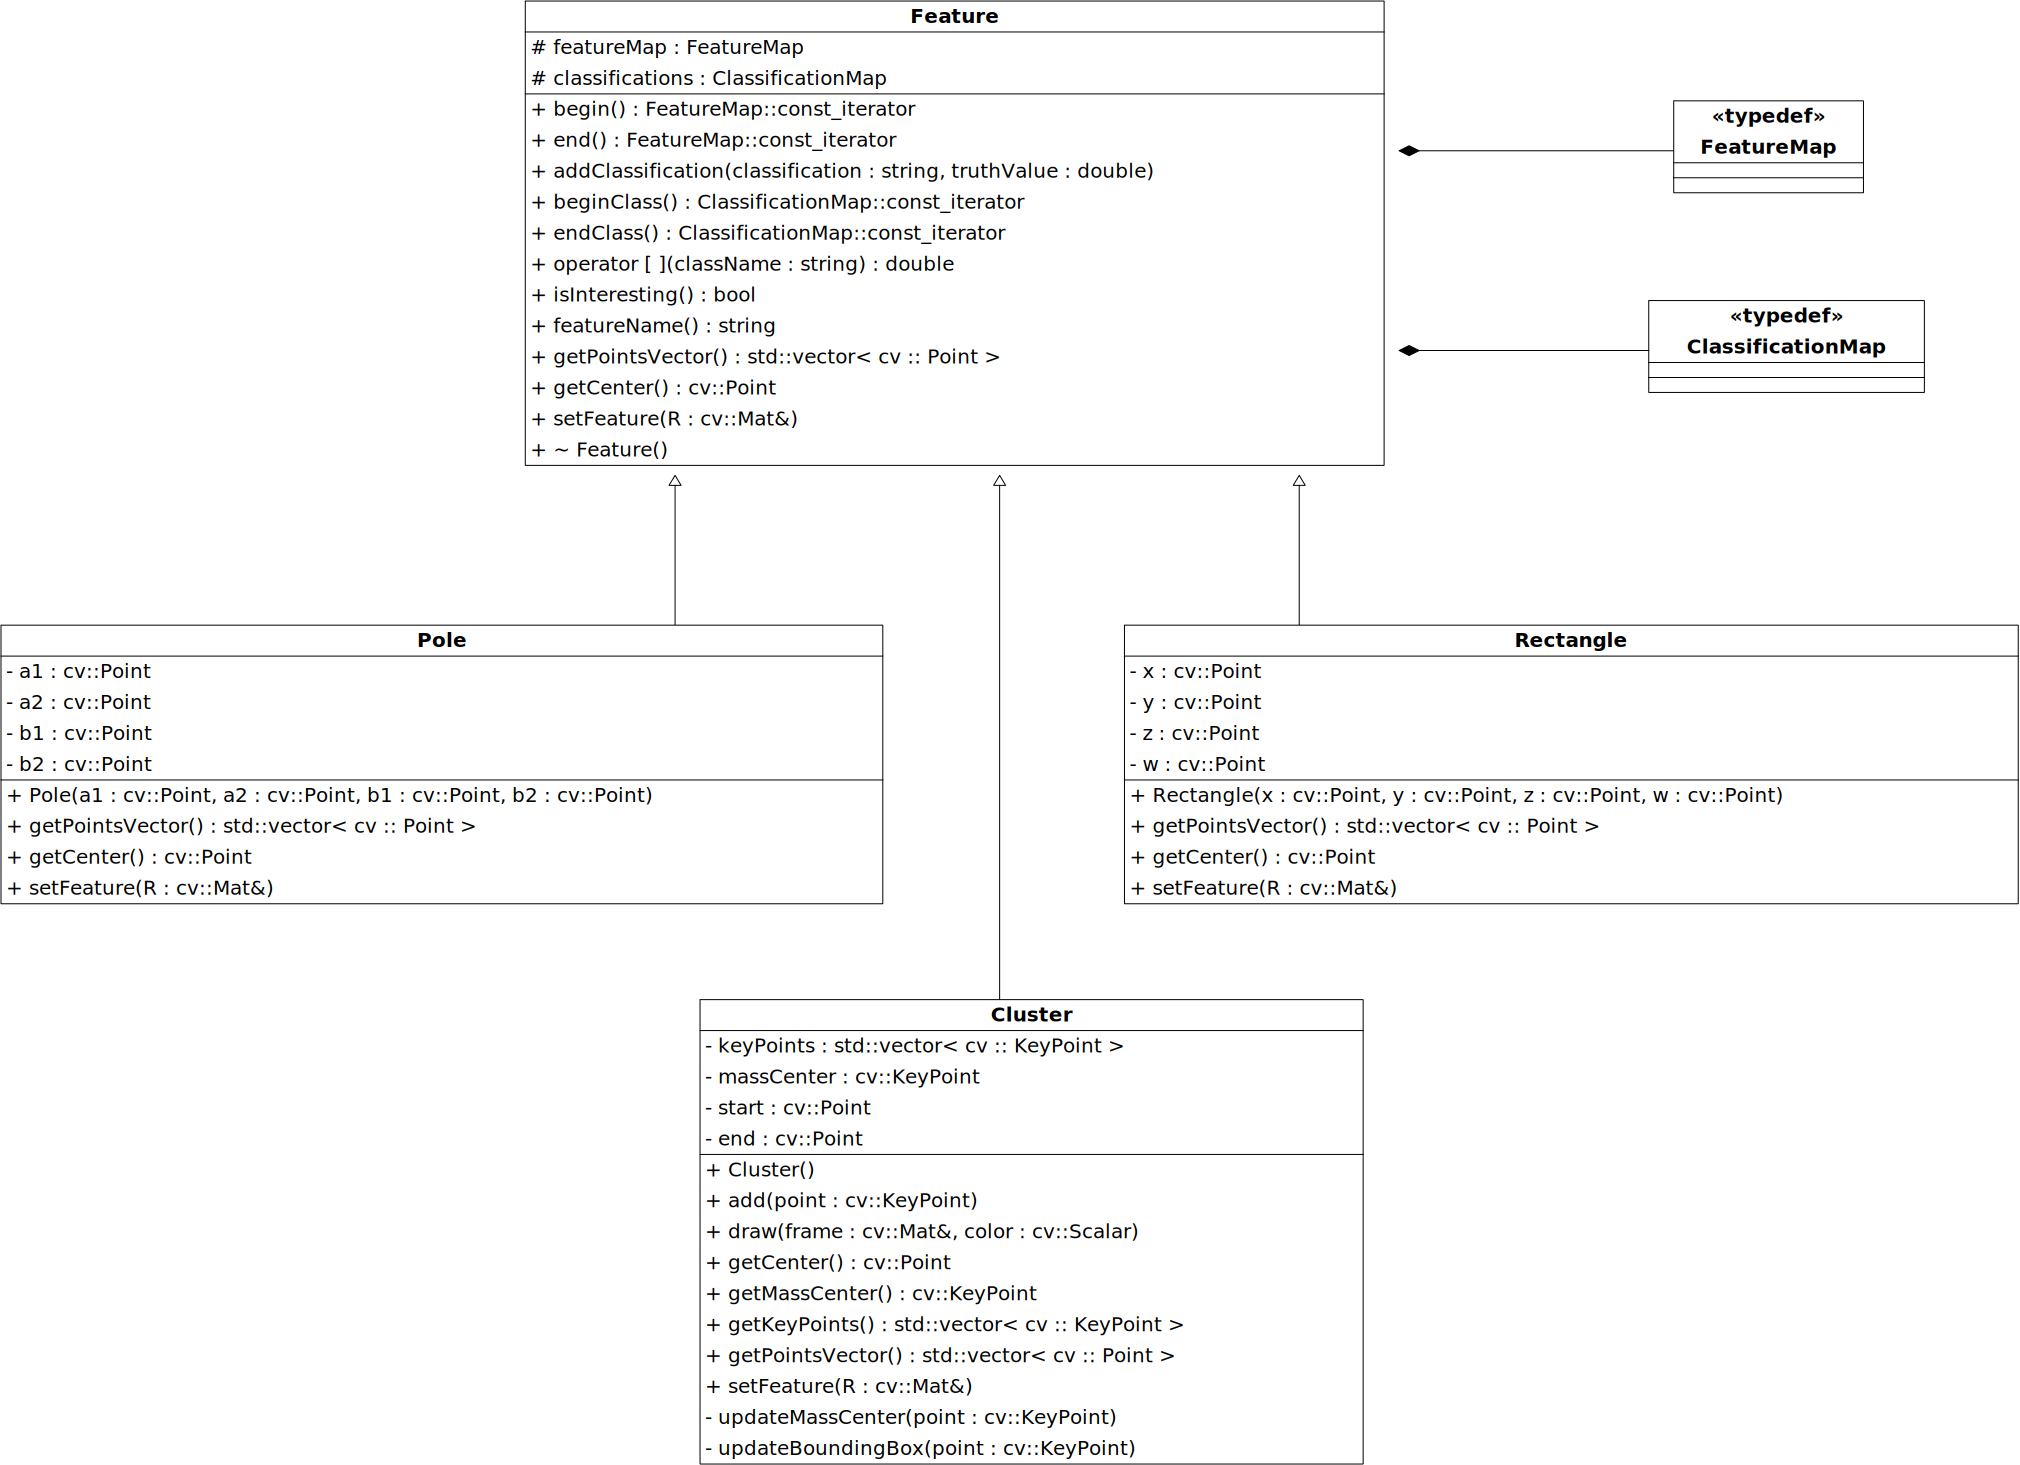
\includegraphics[width=\textwidth]{diagrammi/Feature}
  \caption{Classe Feature e sottoclassi implementate}
  \label{fig:feature}
\end{figure}

Di seguito vengono discussi gli algoritmi implementati per il riconoscimento delle feature geometriche.
La base di partenza per tutti gli algoritmi considerati è l'immagine rettificata della telecamera, ossia l'immagine senza la distorsione causata dalle caratteristiche costruttive della lente, ovvero la distorsione radiale e tangenziale.

\subsection{Quadrilateri}

L'algoritmo di riconoscimento di quadrilateri si basa principalmente sull'algoritmo di Canny~\cite{4767851} per il riconoscimento dei bordi e sulla trasformata di Hough probabilistica~\cite{matas2000robust} per estrarre le linee, o più precisamente, i segmenti, dalla mappa dei bordi.

Le linee estratte contengono, quando l'ambiente è minimamente complesso, molte linee spurie. Inoltre, i quadrilateri interessanti sono composti da due linee approssimativamente orizzontali e due linee approssimativamente verticali. Per questo è stato implementato un algoritmo di filtraggio delle linee in grado di discriminare le linee orizzontali da quelle verticali e dal rumore. Per valutare l'orientamento assoluto delle linee si utilizza la posa del robot. Conoscendo infatti la posa del robot approssimativamente, data l'odometria, è possibile stimare l'inclinazione dell'orizzonte e della linea perpendicolare ad esso. Le linee orizzontali e verticali sono quelle la cui inclinazione, espressa in angolo rispetto all'asse delle ascisse, non supera una determinata soglia rispetto all'orizzonte e alla sua perpendicolare.

Una volta riconosciute le linee verticali e orizzontali viene applicato l'\autorefA{alg:quad-det} per riconoscere quadrilateri e pali.
Viene considerato palo una coppia di linee con un fattore di forma estremamente schiacciato verticalmente. Nell'algoritmo descritto V rappresenta il vettore di linee verticali (ordinate da destra a sinistra), H l'insieme delle linee orizzontali, Q l'insieme di quadrilateri trovati.

\begin{algorithm}[ht]
\caption{QuadrilateralDetector}
\begin{algorithmic}[1] 
\label{alg:quad-det}
\FOR{$i \in \lbrace 0, VerticalLinesNumber -1 \rbrace$}
  \STATE $v_{1} \leftarrow V[i]$
  \STATE $v_{2} \leftarrow V[i+1]$
  \IF{$v_{1}$ and $v_{2}$ are not poles}
    \FORALL{$(h_{1},h_{2}) \in H \times H$}
      \STATE $x \leftarrow$ findInterception($h_{1}$, $v_{1}$);
      \STATE $y \leftarrow$ findInterception($h_{1}$, $v_{2}$);
      \STATE $z \leftarrow$ findInterception($h_{2}$, $v_{2}$);
      \STATE $w \leftarrow$ findInterception($h_{2}$, $v_{1}$);
      \IF{$x,y,z,w$ are the vertices of a quadrilateral $q$}
	\STATE $Q = Q \cup \lbrace q \rbrace$
      \ENDIF
    \ENDFOR
  \ENDIF
\ENDFOR
\RETURN Q
\end{algorithmic}
\end{algorithm}

Questo algoritmo si basa su una considerazione fondamentale per ridurre la complessità del calcolo, ossia che è altamente probabile che un rettangolo interessante si trovi tra due linee verticali consecutive. Questa considerazione è sostenuta dal fattore di forma dell'immagine, che è largo, e dal fattore di forma della maggior parte dei quadrilateri interessanti, che solitamente sono più stretti che larghi. Questa considerazione non si può tuttavia estendere al caso delle linee orizzontali, per le motivazioni opposte, e per questo la ricerca è fatta in maniera esaustiva.


Per discriminare se un insieme di punti formano o meno un quadrilatero vengono utilizzate due euristiche, a seconda del riconoscimento effettuato.
L'euristica più semplice consiste nel considerare tutto ciò che non è un palo come un quadrilatero. Questa euristica in generale è pessima, ma funziona molto bene, avendo un tasso di recupero decisamente alto, quando il riconoscimento è localizzato.

L'altra euristica possibile che abbiamo sviluppato consiste nello sfruttare le proprietà delle combinazioni convesse. Una combinazione convessa è definita come una combinazione lineare con coefficienti positivi e la cui somma vale 1. L'insieme delle combinazioni convesse di un insieme di punti generano l'involucro convesso dell'insieme.
Nel nostro caso, preso un segmento riconosciuto come possibile lato del quadrilatero, possiamo calcolare qualsiasi punto al suo interno tramite la formula:

\begin{equation}
  x = \alpha\cdot a + (1 - \alpha)\cdot b = b + \alpha\cdot(a - b)
\end{equation}

Dove $a$ e $b$ sono gli estremi del segmento e $x$ è un punto al suo interno, i coefficienti di combinazione convessa sono $\alpha$ e $1 - \alpha$.
Come si nota dalla formula $\alpha = 0$ se $x \equiv b$ e $\alpha = 1$ se $x \equiv a$.
Idealmente, per i vertici di un quadrato, si avrà $\alpha=1$ o $\alpha=0$ se si calcola il coefficiente del vertice rispetto ai due segmenti adiacenti.

Se si prova a calcolare il valore di $\alpha$ con la stessa formula per un punto fuori dal segmento si ottiene un valore maggiore di uno o minore di zero.

L'euristica proposta si basa sulle considerazioni fatte sopra, supponendo che a causa del rumore e altri fattori, i vertici del quadrato riconosciuto si possano trovare all'interno o all'esterno del segmento. Viene quindi calcolato il valore di combinazione convessa di ciascun vertice e, fissata una soglia, viene riconosciuto come quadrato solo un insieme di segmenti i cui vertici hanno $\alpha=1$ o $\alpha=0$, a meno della soglia.

\subsection{Cluster}

I cluster vengono riconosciuti estraendo i keypoint dall'immagine tramite l'algoritmo FAST~\cite{rosten_2006_machine}.

%% TODO due parole su cos'e' un keypoint. Non e' necessario descrivere FAST, ma magari, a livello di DBSCAN qui sotto...

Una volta estratti i keypoint, vengono estratti i cluster interessanti tramite l'algoritmo DBSCAN~\cite{ester1996density}.
DBSCAN è un algoritmo che si basa sulla distanza tra i punti. Due punti vengono considerati vicini se la distanza tra di loro è minore di una determinata soglia. Vengono quindi inseriti in un unico cluster tutti i punti che sono raggiungibili tramite la relazione di vicinanza. Ciò significa che tutti i vicini di un punto sono inseriti nello stesso cluster, e allo stesso modo i vicini dei vicini, ricorsivamente.
I cluster che non hanno abbastanza punti al loro interno vengono scartati e considerati come rumore.

\section{Integrazione con il reasoning}
Una volta riconosciute le feature interessanti, vengono calcolati i descrittori di tali feature. I descrittori delle feature vengono inseriti nella FeatureMap, per poter comunicare la feature riconosciuta al classificatore fuzzy.
Viene effettuata la rotazione delle coordinate in modo da avere i quadrilateri riconosciuti il più possibile orientati verticalmente. Questo facilita il compito del reasoner, in quanto attualmente l'operatore ``on'' supporta solo intervalli semplici e non aree o intervalli generici (si veda \autoref{cap:reasoning}).
Le richieste di classificazione vengono, per quanto possibile, inviate contemporaneamente al reasoner, in modo da rendere possibile l'analisi delle relazioni tra gli oggetti riconosciuti. Viene poi popolata, con i dati provenienti dal reasoner, la ClassificationMap. Questo è reso possibile perché ogni feature inviata è associata a un indice univoco.
%%TODO Questo e' un po' confuso. Magari 2 parole in piu' aiuterebbero


\section{Livelli di riconoscimento}
Il riconoscimento degli oggetti non è effettuato tramite una singola analisi dell'immagine, ma viene effettuato su più livelli, sfruttando tutte le informazioni possibili.

Il riconoscimento di basso livello estrae possibili feature dall'immagine intera, in modo che le feature riconosciute possano essere seguite dal tracker. Poiché è importante escludere i falsi positivi il più possibile, e poiché è più complesso analizzare una intera immagine senza conoscere a priori la posizione degli oggetti interessanti, il riconoscimento di basso livello è molto restrittivo. L'euristica utilizzata per riconoscere i quadrilateri nell'immagine è quella che sfrutta le proprietà della combinazione convessa.
Per rendere la computazione più semplice e rapida, non vengono estratti cluster dall'immagine, e le uniche feature analizzate dal reasoner sono i quadrilateri che rappresentano possibili rettangoli.

Una volta riconosciuti i possibili rettangoli interessanti, gli oggetti vengono quindi seguiti dal tracker. Grazie alle informazioni del tracker, descritte nel \autoref{cap:tracking}, è possibile effettuare un'analisi degli oggetti più localizzata. Questo permette un'analisi dell'immagine più semplice, ed è quindi possibile utilizzare tecniche meno discriminative e più robuste. Usiamo quindi l'euristica più semplice (tutto è un quadrilatero) e estraiamo cluster solo in prossimità della regione di interesse, in modo da risparmiare potenza computazionale sia durante l'estrazione delle feature, sia durante il reasoning, eliminando gli oggetti incorrelati. Questa ultima fase quindi è in grado di analizzare feature complesse come gli oggetti composti da più parti, ad esempio le porte.
%%TODO anche questa ultima frase e' forse tropo sintetica e non si capisce cosa fa

%%TODO Mettere all'inizio il fatto che si vuole fare tutto quello che si fa in tempo reale, per poterlo usare in navigazione sul robot reale.

\chapter{Tracking}
\label{cap:tracking}
\thispagestyle{empty}

\begin{quotation}
{\footnotesize
\noindent\emph{Marty: Ma allora dove diavolo sono? \\
Doc: La domanda giusta è: 'Quando diavolo sono?'}
\begin{flushright}
Ritorno al Futuro, parte I
\end{flushright}
}
\end{quotation}
\vspace{0.5cm}

\section{Introduzione}

Una volta riconosciute le possibili feature, è necessario seguirle nelle immagini successive della telecamera.
Per farlo ci siamo basati su un algoritmo presente in letteratura, chiamato Consensus-based Matching and Tracking, CMT~\cite{Nebehay2014WACV}.
L'algoritmo considerato è un algoritmo di tracking a lungo termine. Gli algoritmi di tracking a lungo termine permettono di inseguire oggetti che entrano e escono dal campo visivo della telecamera, e cercano di discriminare anche oggetti simili.

Il tracker implementato è in grado non solo di riconoscere gli oggetti nell'immagine, ma è in grado, in parte, di capire se gli oggetti riconosciuti dall'algoritmo descritto nel \autoref{cap:riconoscimento} sono già o meno nella lista delle track.

In questo capitolo spiegheremo brevemente come funziona l'algoritmo CMT utilizzato e come è stato integrato con il riconoscimento di oggetti e con la costruzione della mappa.

\section{CMT}

L'idea base dell'algoritmo è che i keypoint sono un buon modo per scomporre in parti l'oggetto da seguire. Il primo passo consiste quindi nell'estrarre keypoint dal bounding box iniziale, calcolare i relativi descrittori delle feature e salvare tutto in un database. Questa idea è resa possibile dal recente sviluppo di algoritmi veloci ed efficienti per l'estrazione di feature quali~\cite{rosten_2006_machine} e~\cite{6126542}.

Successivamente, per ogni frame, i keypoint presenti nell'iterazione precedente vengono inseguiti tramite il calcolo del flusso ottico~\cite{Lucas:1981:IIR:1623264.1623280} di Lukas-Kanade, nella variante piramidale~\cite{Bouguet00pyramidalimplementation}. Inoltre vengono estratti keypoint e effettuato il matching con i keypoint presenti nel database. I keypoint di cui è stato effettuato con successo il matching vengono sostituiti a quelli seguiti tramite il flusso ottico, poiché si suppone che siano più stabili, non essendo parte di un processo iterativo di valutazione, soggetto ad errore integrale.

La seconda fase consiste in una procedura di votazione per determinare il centro di massa dell'oggetto.
In primo luogo vengono stimate la scala e la rotazione planare dell'oggetto, calcolando la variazione di scala e di rotazione tra tutte le coppie di keypoint e calcolandone la mediana. In seguito ogni keypoint vota il centro di massa dell'oggetto utilizzando la sua posizione relativa al centro di massa nel primo frame, opportunamente scalato e ruotato grazie ai due valori precedentemente calcolati.

La terza fase dell'algoritmo consiste nell'eliminazione degli outlier tramite un meccanismo di consenso. I centri di massa votati da ciascun singolo keypoint vengono divisi in cluster in base alla distanza euclidea. Quindi, viene individuato il cluster con il maggior numero di voti. Se il cluster scelto ha un numero sufficiente di keypoint, allora l'oggetto viene considerato come visibile e viene calcolato il centro di massa dell'oggetto, eliminando tutti i voti che non appartengono al cluster.

Infine il bounding box dell'oggetto viene calcolato applicando la rotazione e la scala calcolate precedentemente ai punti del bounding box iniziale. Questo procedimento è il punto più debole dell'algoritmo, perché il bounding box calcolato non tiene conto dell'omografia che può esserci tra il bounding box iniziale e quello attuale, causata, ad esempio, dalla distorsione prospettica a seguito della nuova posa della telecamera.

La nostra implementazione si discosta dall'implementazione originale, su cui è fortemente basata, solo per la possibilità di specificare un bounding box con una forma arbitraria.

\section{Integrazione con il riconoscimento degli oggetti}

L'algoritmo di tracking deve essere in grado di interagire con il riconoscimento a basso e alto livello degli oggetti. Per ottenere questo risultato abbiamo implementato alcune euristiche per gestire a basso livello e in maniera semplice i possibili conflitti tra l'algoritmo di tracking e il riconoscimento.

In primo luogo, per facilitare sia il tracking dell'oggetto, sia il riconoscimento ad alto livello, quando il tracker considera un nuovo oggetto da seguire inviato dal riconoscimento a basso livello, non utilizza il bounding box esatto riconosciuto, ma viene maggiorato, scalandolo, in modo da ottenere due importanti risultati:

\begin{enumerate}
 \item Riuscire a riconoscere in maniera efficiente i keypoint che si trovano sui bordi degli oggetti, che spesso sono i keypoint più significativi, soprattutto negli oggetti planari e uniformi, principali obbiettivi di questa tesi.
 \item Riuscire a compensare parzialmente il problema causato dal cambio di posa della telecamera, che potrebbe causare la fuoriuscita dell'oggetto, o parte di esso, dal bounding box, a causa della deformazione prospettica, non calcolata dall'algoritmo.
\end{enumerate}

Le track inviate al riconoscimento di alto livello comprendono due informazioni: il bounding box (maggiorato) e la regione di interesse rettangolare che lo contiene. Questo permette al riconoscimento di alto livello di analizzare solo le regioni di interesse rettangolari dell'immagine, rendendo il compito meno oneroso computazionalmente e di cancellare eventuali feature esterne all'oggetto, che non sono di interesse per il riconoscimento.

L'ultimo problema riguardante l'integrazione, il più problematico, è riuscire a discriminare quali oggetti riconosciuti sono già presenti nella lista delle track.

Questo problema può essere risolto a due livelli. Ad alto livello, è possibile capire che due oggetti trackati nella mappa occupano lo stesso spazio, e quindi fanno parte dello stesso oggetto. Questa soluzione è la soluzione ottimale, ma richiede un maggior numero di informazioni e un costo computazionale maggiore. 
Tuttavia è possibile affrontare parzialmente il problema a basso livello, escludendo in maniera semplice gli oggetti riconosciuti.
L'euristica che abbiamo sviluppato si basa sul calcolo della posizione del centro di massa degli oggetti riconosciuti e delle track, rispetto ai loro bounding box.
Se un oggetto riconosciuto ha il suo centro di massa all'interno di un bounding box di una track attiva, o, viceversa, se una track attiva ha il suo centro di massa nel bounding box dell'oggetto riconosciuto, tale oggetto è considerato già seguito, e non viene aggiunto alla lista delle track.

Come si può vedere dalla figura, %%TODO figura
l'euristica copre abbastanza bene quasi tutti i casi, a parte quando si tratta di oggetti composti da più oggetti o oggetti che si trovano di fronte ad altri oggetti. Per questi casi sono necessarie due ragionamenti ad alto livello differenti: riuscire a capire che un oggetto è semanticamente composto da alcune parti; riuscire a capire che i due oggetti non occupano lo stesso spazio. Per entrambi i ragionamenti non bastano le informazioni estratte dalla singola immagine.

\section{Integrazione con la mappa}
%%TODO non è implementato nulla di quello che c'è scritto in questa sezione. devo toglierlo? l'idea c'è...
L'euristica descritta nel paragrafo precedente dimostra comportarsi molto bene nelle situazioni reali, tuttavia subentrano alcuni problemi quando il tracking degli oggetti presenta dei mancati riconoscimenti. Questo causa spesso la sovrapposizione di più track dello stesso oggetto. Questo problema si può risolvere solamente integrando l'algoritmo di tracking con la mappa degli oggetti riconosciuti. Tramite la mappa è facile accorgersi che lo stesso oggetto è seguito più volte, poiché occupa la stessa posizione dell'oggetto seguito in precedenza.

Il tracking degli oggetti è un compito abbastanza oneroso computazionalmente. Se la posizione del robot è nota, anche in maniera imprecisa, non è necessario mantenere attivo l'algoritmo di tracking per tutti gli oggetti. Inoltre l'algoritmo usato è soggetto a falsi positivi; potendo filtrare le track che non possono essere attive, perché non si trovano nell'area vista dal robot in un determinato istante, il rate di falsi positivi cala drasticamente.

Infine grazie alla stima della posizione, si può calcolare l'omografia che tiene conto della deformazione prospettica del bounding box dell'oggetto rispetto al nuovo punto di vista. Così facendo si può facilitare il riconoscimento ad alto livello.



\cleardoublepage
% ---- Bibliography ----
\addcontentsline{toc}{chapter}{Bibliografia}
\bibliographystyle{plain}
\bibliography{bibl_tesi}
%\nocite{*}

\appendix

\pagestyle{fancy} 
\fancyfoot{}                                               
\renewcommand{\chaptermark}[1]{\markboth{\appendixname\ \thechapter.\ #1}{}} 
\renewcommand{\sectionmark}[1]{\markright{\thesection.\ #1}}         
\fancyhead[LE,RO]{\bfseries\thepage}    
                                        
\fancyhead[RE]{\bfseries\leftmark}    
\fancyhead[LO]{\bfseries\rightmark}     
\renewcommand{\headrulewidth}{0.3pt} 

\chapter{Documentazione del progetto logico}
\label{appendiceA}
\thispagestyle{empty}

\noindent Documentazione del progetto logico dove si documenta il progetto logico del sistema e se \`e il caso si mostra la progettazione in grande del SW e dell'HW. Quest'appendice mostra l'architettura logica implementativa (nella Sezione 4 c'era la descrizione, qui ci vanno gli schemi a blocchi e i diagrammi).
\chapter{Esempio di impiego}
\label{appendiceE}
\thispagestyle{empty}

\noindent Un esempio di impiego del sistema realizzato.
\chapter{Listato}
\label{appendiceC}
\thispagestyle{empty}

\noindent Il listato (o solo parti rilevanti di questo, se risulta particolarmente esteso) con l'autodocumentazione relativa.
\chapter{Il manuale utente}
\label{appendiceD}
\thispagestyle{empty}

\noindent Manuale utente per l'utilizzo del sistema
\chapter{Esempio di impiego}
\label{appendiceE}
\thispagestyle{empty}

\noindent Un esempio di impiego del sistema realizzato.
\chapter{Datasheet}
\label{appendiceF}
\thispagestyle{empty}

\noindent Eventuali Datasheet di riferimento.

\end{document}





